\chapter{Implementation}\label{Chap:Impl}
\section{Used technologies}
\begin{figure}[!htb]
   \centering
   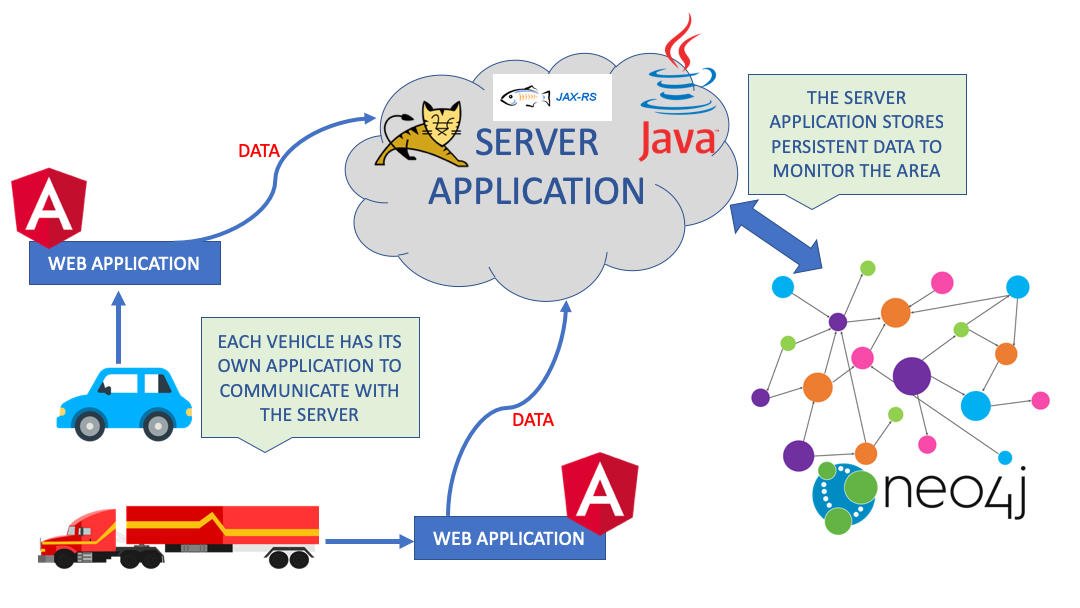
\includegraphics[width=\textwidth]{architecture_impl.png}
   \caption{Architecture of the system with which technologies have been used for each component.}\label{Fig:ArchImpl}
\end{figure}
In figure \ref{Fig:ArchImpl} are presented the various components of the system along with the technologies used to achieve the objectives of each one. In particular:
\begin{itemize}
  \item for the \underline{server} application have been used various technologies:
    \begin{enumerate}
      \item \textbf{Apache Tomcat} is an open source software that implements a \textit{web server}, i.e. it manages the handling of Java Servlets, JSP. It is used to deploy web applications developed in Java \parencite{tomcat}.
      \item \textbf{JAX-RS} has been used as a framework to develop REST application, given the used language has been \textbf{Java}.
    \end{enumerate}
  \item for the \underline{database} component it has been decided to use \textbf{Neo4j} as
    storage for persistent data. Since what we are operating on (a map of places) can be modelled as connection between nodes, Neo4j, as a graph database, came in handy. Also it allowed to specify the type of relations between different nodes in the database as discussed in chapter \ref{Chap:Neo4j}.
  \item client -- TODO
\end{itemize}

% --------------------------------------------------------------------------

\section{Communication between components}
There are two communicationchannels in this architecture:
\begin{enumerate}
  \item cleint $\leftrightarrow$ server:he server is able to speak both XML and JSON, but for this particular project has been decided to use mainly JSON;
  \item server $\leftrightarrow$ database: in this case the server uses \textbf{Cypher} query language (specific for Neo4j) in order to run queries in the database. As a result it is obtained a pseudo-json from which it is possible to extract the desired data, asked in the query.
\end{enumerate}

% --------------------------------------------------------------------------
